\documentclass{standalone}
\usepackage{tikz}
\usetikzlibrary{patterns, positioning}
\usepackage[sfdefault]{ClearSans} %% option 'sfdefault' activates Clear Sans as the default text font
\usepackage[T1]{fontenc}

\begin{document}
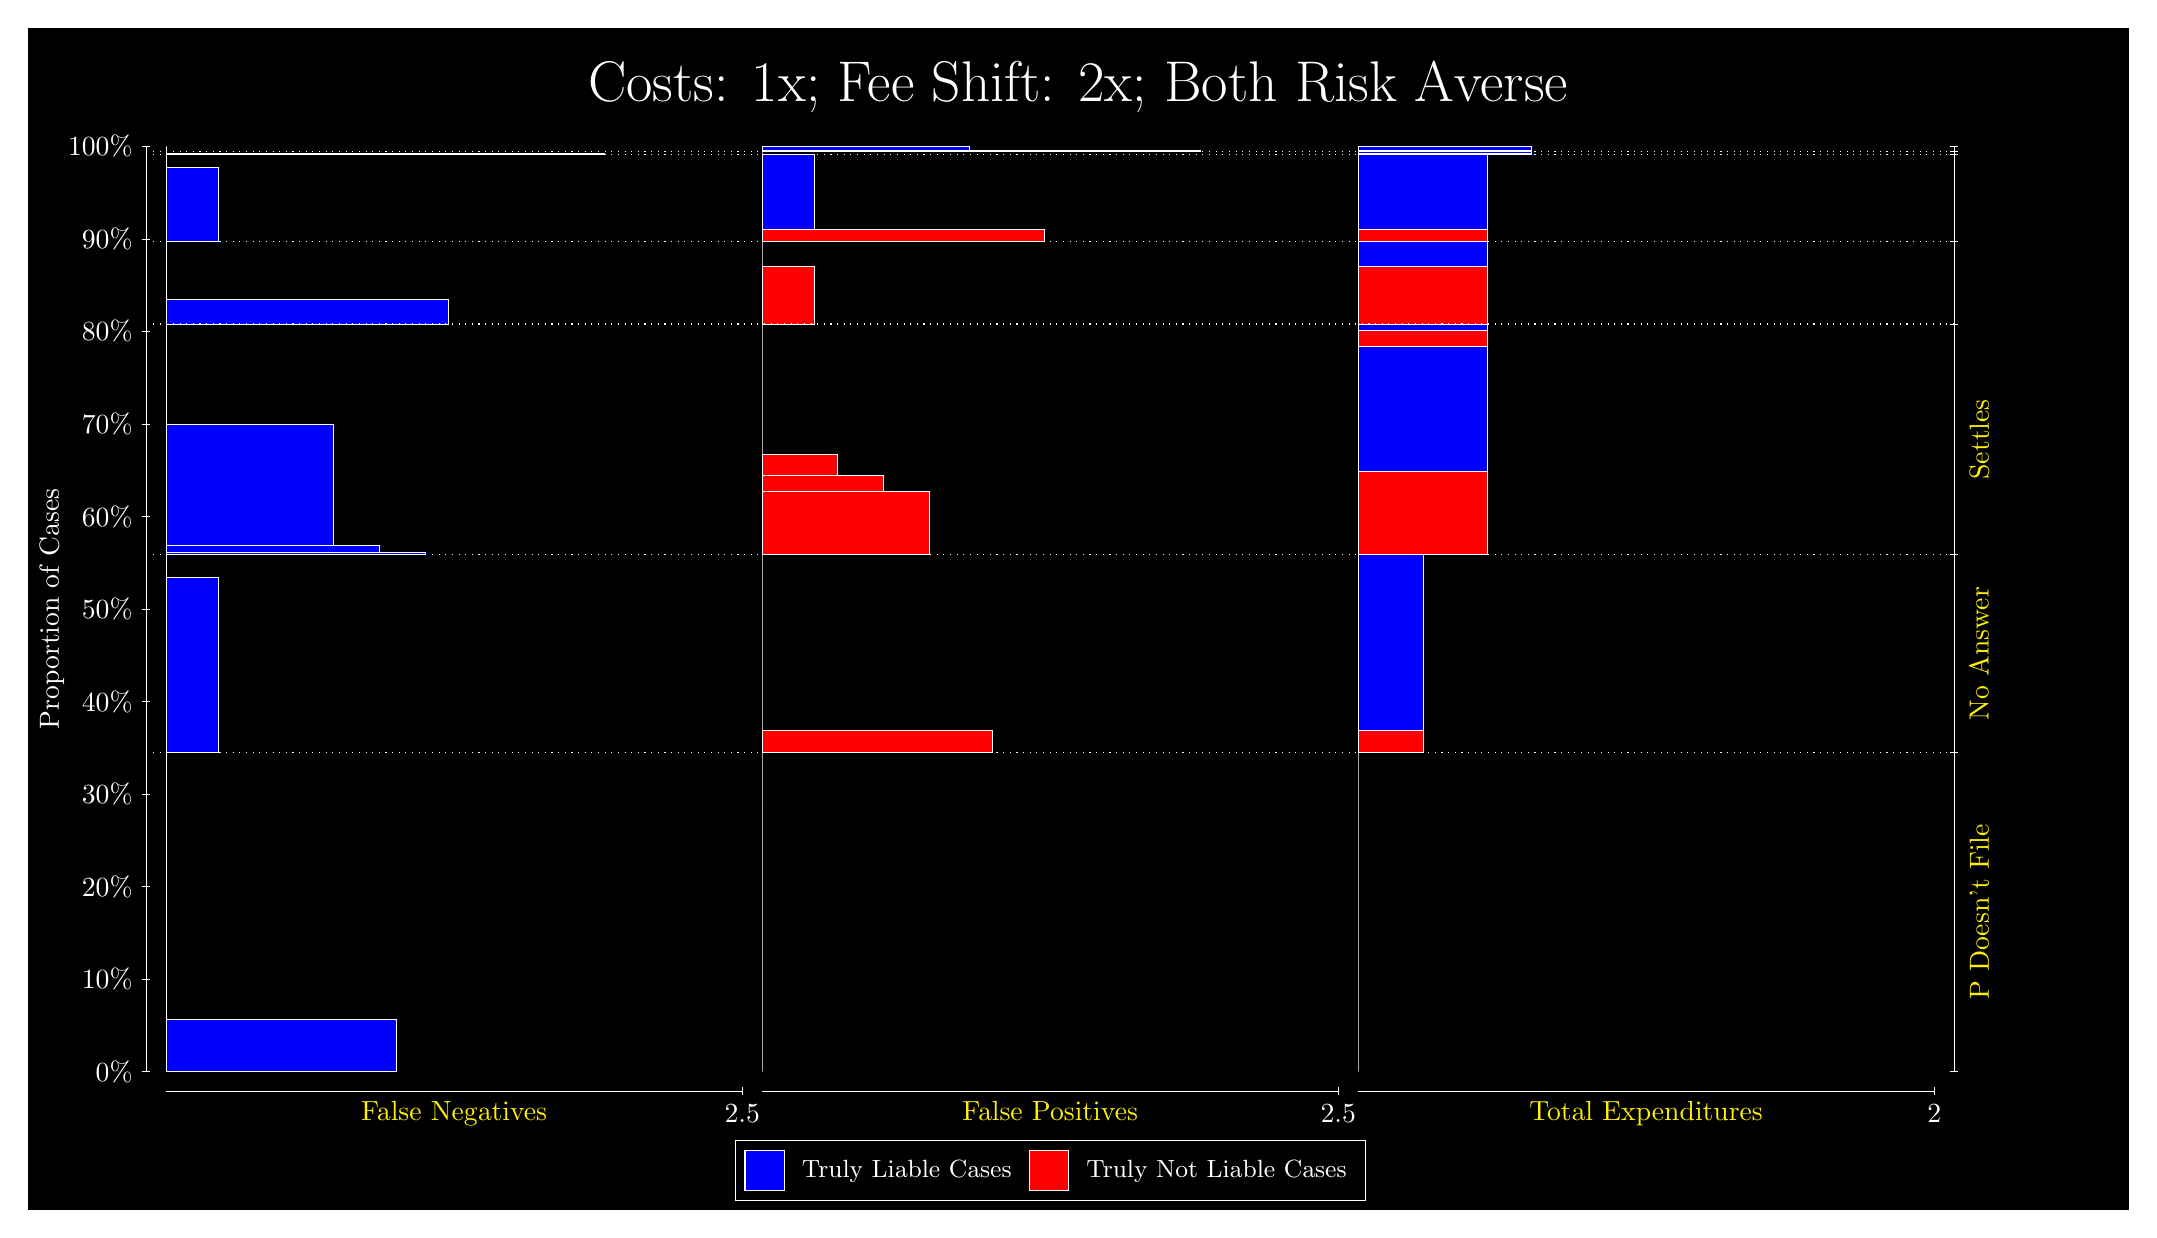
\begin{tikzpicture}
\draw[fill=black] (0,0) rectangle (26.667,15);
\draw[text=white] (0,13.5) rectangle (26.667,15) node[midway] {\huge Costs: 1x; Fee Shift: 2x; Both Risk Averse};
\draw[white, very thin] (1.5,1.75) -- (1.5,13.5);
\node[rotate=90, text=white, anchor=center] at (0.3, 7.625) {Proportion of Cases};
\draw[white, very thin] (1.45,1.75) -- (1.55,1.75);
\node[text=white, anchor=east] at (1.45, 1.75) {0\%};
\draw[white, very thin] (1.45,2.925) -- (1.55,2.925);
\node[text=white, anchor=east] at (1.45, 2.925) {10\%};
\draw[white, very thin] (1.45,4.1) -- (1.55,4.1);
\node[text=white, anchor=east] at (1.45, 4.1) {20\%};
\draw[white, very thin] (1.45,5.275) -- (1.55,5.275);
\node[text=white, anchor=east] at (1.45, 5.275) {30\%};
\draw[white, very thin] (1.45,6.45) -- (1.55,6.45);
\node[text=white, anchor=east] at (1.45, 6.45) {40\%};
\draw[white, very thin] (1.45,7.625) -- (1.55,7.625);
\node[text=white, anchor=east] at (1.45, 7.625) {50\%};
\draw[white, very thin] (1.45,8.8) -- (1.55,8.8);
\node[text=white, anchor=east] at (1.45, 8.8) {60\%};
\draw[white, very thin] (1.45,9.975) -- (1.55,9.975);
\node[text=white, anchor=east] at (1.45, 9.975) {70\%};
\draw[white, very thin] (1.45,11.15) -- (1.55,11.15);
\node[text=white, anchor=east] at (1.45, 11.15) {80\%};
\draw[white, very thin] (1.45,12.325) -- (1.55,12.325);
\node[text=white, anchor=east] at (1.45, 12.325) {90\%};
\draw[white, very thin] (1.45,13.5) -- (1.55,13.5);
\node[text=white, anchor=east] at (1.45, 13.5) {100\%};

\draw[white, very thin] (24.457,1.75) -- (24.457,13.5);
\draw[white, very thin] (24.407,1.75) -- (24.507,1.75);
\node[anchor=west] at (24.407, 1.75) {};
\draw[white, very thin] (24.407,5.8023) -- (24.507,5.8023);
\node[anchor=west] at (24.407, 5.8023) {};
\draw[white, very thin] (24.407,8.3144) -- (24.507,8.3144);
\node[anchor=west] at (24.407, 8.3144) {};
\draw[white, very thin] (24.407,11.243) -- (24.507,11.243);
\node[anchor=west] at (24.407, 11.243) {};
\draw[white, very thin] (24.407,12.289) -- (24.507,12.289);
\node[anchor=west] at (24.407, 12.289) {};
\draw[white, very thin] (24.407,13.393) -- (24.507,13.393);
\node[anchor=west] at (24.407, 13.393) {};
\draw[white, very thin] (24.407,13.435) -- (24.507,13.435);
\node[anchor=west] at (24.407, 13.435) {};
\draw[white, very thin] (24.407,13.5) -- (24.507,13.5);
\node[anchor=west] at (24.407, 13.5) {};

\draw[white, very thin, fill=blue] (1.75,1.75) rectangle (4.6775,2.4106);
\draw[white, very thin, fill=red] (1.75,2.4106) rectangle (1.75,5.8023);
\draw[white, very thin, fill=blue] (1.75,5.8023) rectangle (2.4087,8.0283);
\draw[white, very thin, fill=red] (1.75,8.0283) rectangle (1.75,8.3144);
\draw[white, very thin, fill=blue] (1.75,8.3144) rectangle (5.0435,8.3499);
\draw[white, very thin, fill=blue] (1.75,8.3499) rectangle (4.458,8.4282);
\draw[white, very thin, fill=blue] (1.75,8.4282) rectangle (3.8725,9.9733);
\draw[white, very thin, fill=red] (1.75,9.9733) rectangle (1.75,11.243);
\draw[white, very thin, fill=blue] (1.75,11.243) rectangle (5.3362,11.56);
\draw[white, very thin, fill=red] (1.75,11.56) rectangle (1.75,12.289);
\draw[white, very thin, fill=blue] (1.75,12.289) rectangle (2.4087,13.236);
\draw[white, very thin, fill=red] (1.75,13.236) rectangle (1.75,13.393);
\draw[white, very thin, fill=blue] (1.75,13.393) rectangle (7.3123,13.411);
\draw[white, very thin, fill=red] (1.75,13.411) rectangle (1.75,13.435);
\draw[white, very thin, fill=red] (1.75,13.435) rectangle (1.75,13.453);
\draw[white, very thin, fill=blue] (1.75,13.453) rectangle (1.75,13.5);
\draw[white, very thin, fill=red] (9.3189,1.75) rectangle (9.3189,5.1417);
\draw[white, very thin, fill=blue] (9.3189,5.1417) rectangle (9.3189,5.8023);
\draw[white, very thin, fill=red] (9.3189,5.8023) rectangle (12.246,6.0883);
\draw[white, very thin, fill=blue] (9.3189,6.0883) rectangle (9.3189,8.3144);
\draw[white, very thin, fill=red] (9.3189,8.3144) rectangle (11.441,9.1226);
\draw[white, very thin, fill=red] (9.3189,9.1226) rectangle (10.856,9.328);
\draw[white, very thin, fill=red] (9.3189,9.328) rectangle (10.27,9.5836);
\draw[white, very thin, fill=blue] (9.3189,9.5836) rectangle (9.3189,11.243);
\draw[white, very thin, fill=red] (9.3189,11.243) rectangle (9.9776,11.972);
\draw[white, very thin, fill=blue] (9.3189,11.972) rectangle (9.3189,12.289);
\draw[white, very thin, fill=red] (9.3189,12.289) rectangle (12.905,12.446);
\draw[white, very thin, fill=blue] (9.3189,12.446) rectangle (9.9776,13.393);
\draw[white, very thin, fill=red] (9.3189,13.393) rectangle (9.3189,13.417);
\draw[white, very thin, fill=blue] (9.3189,13.417) rectangle (9.3189,13.435);
\draw[white, very thin, fill=red] (9.3189,13.435) rectangle (14.881,13.453);
\draw[white, very thin, fill=blue] (9.3189,13.453) rectangle (11.954,13.5);
\draw[white, very thin, fill=red] (16.888,1.75) rectangle (16.888,5.1417);
\draw[white, very thin, fill=blue] (16.888,5.1417) rectangle (16.888,5.8023);
\draw[white, very thin, fill=red] (16.888,5.8023) rectangle (17.711,6.0883);
\draw[white, very thin, fill=blue] (16.888,6.0883) rectangle (17.711,8.3144);
\draw[white, very thin, fill=red] (16.888,8.3144) rectangle (18.534,9.3782);
\draw[white, very thin, fill=blue] (16.888,9.3782) rectangle (18.534,10.959);
\draw[white, very thin, fill=red] (16.888,10.959) rectangle (18.534,11.164);
\draw[white, very thin, fill=blue] (16.888,11.164) rectangle (18.534,11.243);
\draw[white, very thin, fill=red] (16.888,11.243) rectangle (18.534,11.972);
\draw[white, very thin, fill=blue] (16.888,11.972) rectangle (18.534,12.289);
\draw[white, very thin, fill=red] (16.888,12.289) rectangle (18.534,12.446);
\draw[white, very thin, fill=blue] (16.888,12.446) rectangle (18.534,13.393);
\draw[white, very thin, fill=red] (16.888,13.393) rectangle (19.083,13.417);
\draw[white, very thin, fill=blue] (16.888,13.417) rectangle (19.083,13.435);
\draw[white, very thin, fill=red] (16.888,13.435) rectangle (19.083,13.453);
\draw[white, very thin, fill=blue] (16.888,13.453) rectangle (19.083,13.5);
\draw[white, dotted] (1.5,5.8023) -- (24.457,5.8023);
\draw[white, dotted] (1.5,8.3144) -- (24.457,8.3144);
\draw[white, dotted] (1.5,11.243) -- (24.457,11.243);
\draw[white, dotted] (1.5,12.289) -- (24.457,12.289);
\draw[white, dotted] (1.5,13.393) -- (24.457,13.393);
\draw[white, dotted] (1.5,13.435) -- (24.457,13.435);
\draw[white, very thin] (1.75,1.5) -- (9.0689,1.5);
\node[text=yellow, anchor=north] at (5.4094, 1.5) {False Negatives};
\draw[white, very thin] (9.0689,1.45) -- (9.0689,1.55);
\node[text=white, anchor=north] at (9.0689, 1.45) {2.5};

\draw[white, very thin] (9.3189,1.5) -- (16.638,1.5);
\node[text=yellow, anchor=north] at (12.978, 1.5) {False Positives};
\draw[white, very thin] (16.638,1.45) -- (16.638,1.55);
\node[text=white, anchor=north] at (16.638, 1.45) {2.5};

\draw[white, very thin] (16.888,1.5) -- (24.207,1.5);
\node[text=yellow, anchor=north] at (20.547, 1.5) {Total Expenditures};
\draw[white, very thin] (24.207,1.45) -- (24.207,1.55);
\node[text=white, anchor=north] at (24.207, 1.45) {2};

\node[text=yellow, centered, rotate=90] at (24.777, 3.7761) {P Doesn't File};
\node[text=yellow, centered, rotate=90] at (24.777, 7.0583) {No Answer};
\node[text=yellow, centered, rotate=90] at (24.777, 9.7785) {Settles};





\draw (12.978300999999998,1.5) node[draw=none] (baseCoordinate) {};
\begin{scope}[align=center]
        \matrix[scale=0.5, draw=white, below=0.5cm of baseCoordinate, nodes={draw}, column sep=0.1cm]{
            \node[rectangle, draw, minimum width=0.5cm, minimum height=0.5cm, fill=blue] {}; &
            \node[draw=none, font=\small, text=white] (B) {Truly Liable Cases}; &
            \node[rectangle, draw, minimum width=0.5cm, minimum height=0.5cm, fill=red] {}; &
            \node[draw=none, font=\small, text=white] (B) {Truly Not Liable Cases}; \\
            };
\end{scope}

\end{tikzpicture}
\end{document}